% Figure from MATH 591 notes, section 7. Compile with the notes preamble.
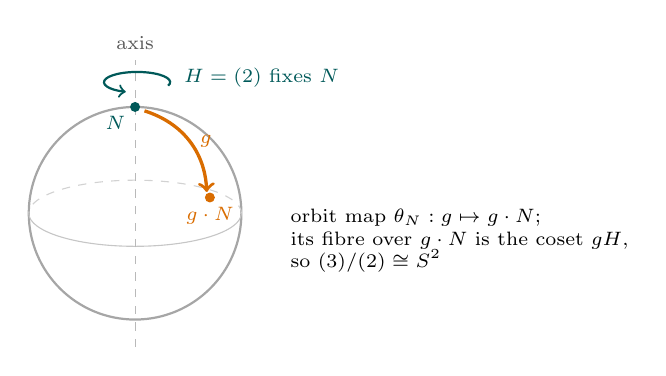
\begin{tikzpicture}
\draw[thick, gray!70] (0,0) circle (1.35); \draw[gray!45] (-1.35,0) arc (180:360:1.35 and 0.42); \draw[gray!35, dashed] (1.35,0) arc (0:180:1.35 and 0.42);
\draw[gray!55, dashed] (0,-1.7) -- (0,1.95) node[above, font=\scriptsize, text=gray!70!black] {axis};
\draw[->, thick, teal!70!black] (0.42,1.62) arc (-20:250:0.42 and 0.13); \node[teal!70!black, font=\scriptsize, anchor=west] at (0.5,1.72) {$H = \SO(2)$ fixes $N$};
\fill[teal!70!black] (0,1.35) circle (1.8pt) node[anchor=north east, font=\scriptsize] {$N$};
\draw[->, very thick, orange!85!black] (0.12,1.3) to[bend left=35] node[right, font=\scriptsize] {$g$} (0.910,0.270);
\fill[orange!85!black] (0.950,0.200) circle (1.8pt) node[anchor=north, font=\scriptsize] {$g \cdot N$};
\node[font=\scriptsize, align=left, anchor=west] at (1.85,-0.35) {orbit map $\theta_N : g \mapsto g\cdot N$;\\ its fibre over $g\cdot N$ is the coset $gH$,\\ so $\SO(3)/\SO(2) \cong S^2$};
\end{tikzpicture}
